%chapter 5
\chapter{Passenger Transport Operation}
%
\section{Public Transportation}
Public transportation is a generic term used to describe the family of transit services available to urban and rural residents. Thus, it is not a single mode but a variety of traditional and innovative services, which should complement each other to provide system-wide mobility.
%
\subsection{Transit Modes}
The modes included within the realm of public transportation are:
\begin{itemize}
	\item \textbf{Mass transit}, characterized by fixed routes, published schedules, designated networks, and specified stops. Mass-transit vehicles include buses, light rail (trolleys) or rapid transit that either share space in mixed traffic or operate on grade-separated rights of way.
	\item \textbf{Paratransit} is characterized by flexible and personalized service intended to replace conventional fixed-route, fixed-schedule mass-transit lines. Paratransit is available to the public on demand, by subscription, or on a shared-ride basis. Examples include taxi, car rental, dial-a-ride, and specialized services for elderly, medical, and other designated users.
	\item \textbf{Ridesharing} (as the name implies) is characterized by two or more persons traveling together by prearrangement, such as carpool, vanpool, or shared-ride taxi.
\end{itemize}
%
\subsection{Transit Capacity and Level of Service}
A basic attribute of any transit mode is its carrying capacity, defined as the number of vehicles or persons that pass a given point in a specified time (usually an hour). The numerical value of carrying capacity (usually referred simply as capacity), is dependent on two variables: (1) the number of vehicles that pass a point at a given time and (2) the number of passengers within each vehicle. For example, if for a given lane along a section of highway there are 60 buses that pass by in an hour (or one per minute), and each bus carries 50 seated passengers, then the carrying capacity of this highway lane is 60 buses/ln/hr or $50 \times 60 = 3000$ passengers/ln/hr.\\
\par
Carrying capacity is influenced by (1) the “spacing” in seconds between each
vehicle (called the headway) and (2) the “comfort factor” experienced by passengers (called the level of service). Thus, carrying capacity can be increased in two ways: (1) reduce the headway or (2) increase the number of passengers per vehicle. In the bus capacity example, the headway was 60 seconds and the level of service was that all passengers had a seat. Time spacing between buses could possibly be reduced, but there are limits to lowering headway values dictated by safe distance requirements between vehicles and/or the time spent at transit stops and terminals (called dwell time). Similarly, passenger loading could be increased by allowing standees, but this would decrease the comfort level for passengers. Were the bus equipped with computer tables and a refreshment area (thus offering a higher level of service), fewer passengers could be accommodated resulting in a lower carrying capacity but a higher level of service.\\
\par
Accordingly, when reporting transit capacity, it is important to specify the units
as either vehicles or passengers/hour and the corresponding level of service in terms of passengers/vehicle. Public transit is often compared with the automobile when issues of carrying capacity are involved, as it is commonly believed that transit capacity is superior to auto capacity. As will be discussed in greater detail in Chapters 9 and 10, the capacity of a single lane of passenger vehicles is approximately 2,000 vehicles/hour which represents a headway of 1.8 seconds. Since most cars have at least five seats, the person capacity of a highway lane could be as great as $ 5 \times 2000 = 10000 $ per/hour. Capacities of this magnitude never have been achieved, since most cars carry only one person with an average car occupancy of about 1.5. Why is this so? Have you ever driven in a car carrying five people? Not a pleasant experience, and a reason why car pooling is not very popular. Given the opportunity, most people choose to drive alone or with just one other person.\\
\par
Travelers usually consider many more factors than simply the in-vehicle level of
service, and they don’t really consider how they can contribute to increasing “carrying capacity.” In fact, if drivers were to optimize the carrying capacity of a highway, they would all drive at 35 miles per hour! Other major considerations in selecting the travel mode include: reliability, punctuality, cost, travel time, and safety. Transit systems that receive “high marks” for the out-of-vehicle level-of-service factors are typically the ones that use exclusive lanes or tracks with no interference from other vehicles or pedestrians and have adequate capacity at station stops and terminals. Thus, rapid transit services (whether bus or fixed guideway), are the superior mode but are more costly to build and maintain and require high volumes of demand to be feasible.
%
\subsection{The Role and Future of Public Transportation}
Public transportation is an important element of the total transportation services provided within large and small metropolitan areas. A major advantage of public transportation is that it can provide high-capacity, energy-efficient movement in densely traveled corridors. It also serves medium- and low-density areas by offering an option for auto owners who do not wish to drive and an essential service to those without access to automobiles, such as school children, senior citizens, single-auto families, and others who may be economically or physically disadvantaged.\\
\par
For most of this century, public transportation was provided by the private sector.
However, increases in auto ownership, shifts in living patterns to low-density suburbs, and the relocation of industry and commerce away from the central city, along with changes in lifestyle (which have been occurring since the end of World War II) have resulted in a steady decline in transit ridership. Since the early 1960s, most transit services have been provided by the public sector. Income from fares no longer represent the principal source of revenue, and over a 25- to 30-year period, the proportion of funds for transit provided by federal, state, and local governments has increased steadily. While it generally is believed that highways and motor transport will play a dominant role in providing personal transportation in the beginning decades of the twenty-first century, there are many unforeseen changes that could alter the balance between public and private transportation. Some could contribute to a decline in transit ridership while others might cause transit to become stronger, and for the remainder, there would be little or no effect. The potential changes that could influence transit usage are categorized here from the book Urban Mass Transportation Planning.
%
\subsubsection{Factors Bad for Transit}
\begin{itemize}
	\item Growth of suburbs
	\item Industry and employment moving from the central city
	\item Increased suburb-to-suburb commuting
	\item Growth in private vehicle ownership
	\item Increased diversity in vehicle types such as SUVs, pickup trucks, and RVs
	\item High labor costs
\end{itemize}
%
\subsubsection{Factors Good for Transit}
\begin{itemize}
	\item Emphasis by the government on air quality
	\item Higher prices of gasoline
	\item Depletion of energy resources
	\item Trends toward higher-density living
	\item Legislation to encourage “livable cities” and “smart growth”
	\item Increased number of people who cannot or choose not to drive 
\end{itemize}
%
\section{Number of Passengers Versus Number of Served Vehicles}
Traffic engineers try by various techniques and measures to enable as many vehicles as possible to pass,
during a specific period of time, through a traffic intersection or through a road section. In other words, traffic experts try to maximize the number ofvehicles that are served during a certain period of time. On the other hand, when it comes to public transit, we are trying to maximize the number of transported passengers. The number of passengers that can be served during the observed time interval represents transit line capacity. Similarly, the number of vehicles that can be served during the observed time interval represents the vehicle line capacity.
\subsection{A Hypothetical Case Study}
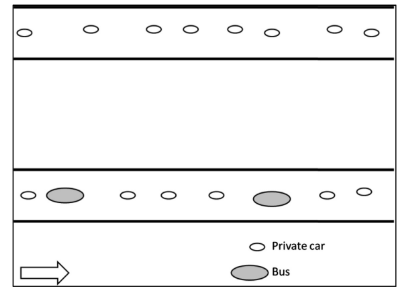
\includegraphics{gfx/fig15.png}\\
Let us assume that the freeway lane can serve 2200 vehicles per hour (the freeway lane capacity equals 2200 vehicles per hour). The upper part of the figure shows the situation when only private cars used freeway lane. The lower part of the figure refers to the situation when some buses also participate in freeway lane traffic. We assume that average number of passengers in bus and private car (average occupancies) are, respectively, equal to 50 and 1.4. We also assume that instead on any two private cars we can allow one bus to participate in freeway lane traffic.\\
\par
We denote by C, B, and P, respectively, the total number of cars, total number of buses, and total number of transported passengers. Ifwe allow, for example, 50 buses to enter the freeway lane, we need to reduce the total number of private cars for $ 50 \times 2 = 100$ private cars.In this case, the total number of transported passengers P by private cars and buses equals:\\\\
$ P = C \times 1.4 + B \times 50 = 2100 \times 1.4 + 50 \times 50 = 5440$ Passengers\\
\par
The table and the graph below show increase in the total number of transported passengers with the increase of the number of buses engaged.\\
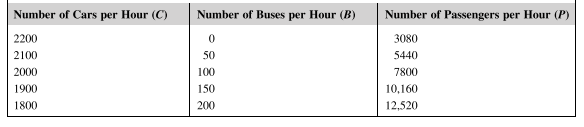
\includegraphics[scale = 0.8]{gfx/fig16.png}\\
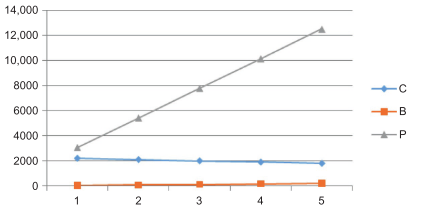
\includegraphics{gfx/fig17.png}\\
%
The graph above illustrates the effects that public transit can achieve. With a very small percentage share of public transport vehicles in the total number of vehicles, it is possible to increase dramatically the total number of passengers carried. To achieve such effects in reality, it is necessary constantly to increase the public transit attractiveness.
%

